%
% Kapitel2.tex
%
\chapter{System Design}
\label{sec:system_design}
In this chapter, the end-to-end system design for capturing, processing, and leveraging phase data for training deep learning model training is presented. The experimental setup used describes the DAS deployment at the Energy Center in Hulb(B\"oblingen), the fiber-optic cable layout, and the HDF5 format~\cite{hdf5} used to archive raw phase measurements. Introduction to a modular data processing pipeline from ingestion and HDF5 file handling, through STFT-based spectrogram generation and logarithmic scaling, to final data serialization illustrated via a block diagram that highlights each stage inputs, outputs, and dependencies. Finally, the model training and testing framework, specifying how ConvNext V2 and EfficientNet will consume these preprocessed spectrograms is outlined.

\section{Experimental Setup for data acquisition}\label{sec:experimental_setup}
Data acquisition represents a fundamental component of this work, and every effort has been made to ensure that the collection process is robust and methodologically sound. The data is gathered using the DAS configurator application, as discussed and elaborated upon in section~\ref{sec:config_app}, it is then downloaded in HDF5 format. The data source is the Energy Building near the AP Sensing main office, where the DAS (Distributed Acoustic Sensing) system is installed. The DAS system, which operates using a state-of-the-art fiber optic cable deployed along a well-defined spatial route, captures walking patterns and other relevant phenomena. Figure~\ref{energiezentrale} illustrates the complete fiber optic cable layout deployed at the Energy Building. This visualization is essential, as it provides context for the subsequent analysis and aids in understanding the spatial distribution of the data.

\begin{figure}[ht]
    \centering
    \includegraphics[width=\linewidth]{Bilder/jpg/energiezentrale.png}
    \caption{Fiber optic layout at the Energy Center \cite{energy_ppt}}
    \label{energiezentrale}
\end{figure}

The fiber-optic cable begins at the AP Sensing office (yellow) and then traverses four segments before reaching Herrenberger Street:

\begin{itemize}
    \item \textbf{Trench near the fence (red, underground):}  
          The cable runs below ground alongside the perimeter fence.
    \item \textbf{Fence line (green, above ground):}  
          The cable is mounted directly onto the fence structure.
    \item \textbf{Distant trench (blue, underground):}  
          The cable returns underground in a trench set back from the fence.
    \item \textbf{Final approach (purple, underground):}  
          The cable continues beneath the ground toward Herrenberger Street.
\end{itemize}

Four numbered junctions mark critical splice and access points (Figure~\ref{energiezentrale}):

\begin{itemize}
    \item \textbf{Junction 1:} Splice box receiving input from the AP Sensing office and feeding out to the building perimeter.
    \item \textbf{Junction 2:} Splice box receiving the perimeter feed and directing it onward toward Herrenberger Street.
    \item \textbf{Junction 3:} Main manhole outside the fence for underground routing.
    \item \textbf{Junction 4:} Smaller pit adjacent to the fence, also used for underground transitions.
\end{itemize}

This layout enables precise spatial localization of acoustic events along the cable route. The footstep data is recorded from the setup by walking around the cable route and logging it properly. DAS system records phase data that reflects variations corresponding to walking patterns. Phase data is stored in an in the HDF5 file in the form of \texttt{xarray} format a multi-dimensional data structure well-suited for handling large, complex datasets. Attributes such as data rate, gauge length, spatial channels  which are set at the time of recording are stored in the HDF5 file in the form of metadata. 

\section{General structure of the system}
\begin{figure}[ht]
    \centering
    % Scale to fit page width
    \resizebox{\textwidth}{!}{%
      \begin{tikzpicture}[
        node distance=0.4cm and 0.6cm,
        >=Stealth,
        block/.style={
          rectangle,
          draw,
          rounded corners,
          text centered,
          minimum width=1.4cm,
          minimum height=0.9cm,
          font=\small,
          fill=gray!10
        }
      ]
      % Define nodes in a single row
      \node[block] (acq) {DAS Acquisition};
      \node[block, right=of acq] (extract) {Extraction};
      \node[block, right=of extract] (preproc) {Preprocessing};
      \node[block, right=of preproc] (dataset) {Dataset Creation};
      \node[block, right=of dataset] (train) {Training};
  
      % Draw arrows
      \draw[->] (acq) -- (extract);
      \draw[->] (extract) -- (preproc);
      \draw[->] (preproc) -- (dataset);
      \draw[->] (dataset) -- (train);
      \draw[->, dotted] (train.north) -- ++(0,1) -| (acq.north);
    \end{tikzpicture}%
    }
    \caption{Block diagram of the general structure of the system}
    \label{fig:footstep-pipeline}
  \end{figure}
  
  Figure~\ref{fig:footstep-pipeline} illustrates the general structure of the system what the thesis is trying to achieve. The system captures the data using the DAS system from the Energy building as explained in section~\ref{sec:experimental_setup}. The walking data is recorded by taking into the consideration the layout of the cable and logging needs to be done properly to determine the exact time and spatial location along the cable where the footsteps are recorded. 

  The data is stored in the HDF5 format which stores the phase data with timestamps and the spatial locations. The footstep data is extracted from the HDF5 file and needs to be stored separately which is needed for training the model. Also, different types of background noise needs to be extracted from the HDF5 file which is needs for the model training. For clear distinction between the footsteps ans background data the data is preprocessed (section~\ref{sec:preprocessing}) and converted into spectrograms. The spectrograms are then used to create the dataset which is used for training the model. The spectrograms are used as the clear distinction between footsteps and background noise can be seen in the spectrograms. Using these spectrograms the model is trained and evaluation is done based on the accuracy of the model. 
  
\section{Internal Structure}
Internally the structure of the system is split into various blocks as shown in Figure~\ref{fig:footstep-pipeline}. The blocks are explained in detail in the following sections. The blocks are designed in such a way that they can be used independently and can be reused for other applications as well. Each block from Figure~\ref{fig:footstep-pipeline} has further smaller blocks which are explained in the following sections. 

\subsection{Data Acquisition}\label{sec:data_acquisition}
In the section~\ref{sec:experimental_setup} it is explained how the fiber optic cable is laid and using the DAS configurator application the data is recorded. The data is stored in the HDF5 format which is a file format used to store large amounts of data. Figure~\ref{fig:daq-simple} gives the overview of data acquisition process. The data acquisition block is the main block from Figure~\ref{fig:footstep-pipeline} which records the data from the DAS setup using the DAS configurator application and stores it in the HDF5 file format. The phase data from this HDF5 file further visualized using the RGB array.

\begin{figure}[ht]
  \centering
  \resizebox{\textwidth}{!}{%%
    \begin{tikzpicture}[
      node distance=1cm,
      >=Stealth,
      subblock/.style={
        rectangle,
        draw,
        rounded corners,
        text centered,
        minimum width=2.5cm,
        minimum height=0.8cm,
        font=\scriptsize,
        fill=blue!10,
      },
      container/.style={
        rectangle,
        draw,
        thick,
        rounded corners,
        fill=gray!20,
      }
    ]
    % Layers
    \pgfdeclarelayer{background}
    \pgfsetlayers{background,main}

    % Sub-blocks
    \node[subblock] (rec) {Recording};
    \node[subblock, right=of rec] (hdf) {HDF5 Storage};
    \node[subblock, right=of hdf] (viz) {Visualization};

    % Draw arrows
    \draw[->] (rec) -- (hdf);
    \draw[->] (hdf) -- (viz);

    % Container in background
    \begin{pgfonlayer}{background}
      \node[container, fit=(rec) (hdf) (viz), inner sep=10pt] (daq) {};
      \node[anchor=north west, font=\scriptsize] at (daq.north west) {Data Acquisition};
    \end{pgfonlayer}
  \end{tikzpicture}%%
  }
  \caption{Data acquisition block: Recording phase data, storing in HDF5 format, and visualizing the data.}
  \label{fig:daq-simple}
\end{figure}
The data in HDF5 file is stored in the form of xarray format. The xarray format is a multi-dimensional data structure that allows for easy manipulation and analysis of large datasets. The phase data is stored in the HDF5 file with timestamps and the distance along the cable route at which the data is recorded. For better viewing the data is converted into a DataFrame which is a tabular format~\cite{mckinney2010data}. DataFrame contains the phase data with timestamps and the distance along the cable route at which the data is recorded. Table~\ref{tab:phase_data} shows the phase data in the form of a matrix with the distance along the cable route on the x-axis and time on the y-axis. Each cell in the table represents the phase data at a specific distance and time. 

\begin{table}[ht]
  \centering
  \resizebox{\textwidth}{!}{%
    \begin{tabular}{l r c r c r}
      \toprule
      & \multicolumn{5}{c}{\textbf{Distance (m)}} \\
      \cmidrule(lr){2-6}
      \textbf{Timestamps (UTC)} 
        & 53638.285156 & \dots & 53701.992188 & \dots & 53726.496094 \\
      \midrule
      2024-10-21 10:27:40.000183+00:00 
        &   243.9019   & \dots & 1105.7420    & \dots &   854.9858    \\
      2024-10-21 10:27:40.001183+00:00
        &  -908.2096   & \dots & -3462.1868   & \dots &  2459.3839    \\
      \vdots 
        &   \vdots     &       &  \vdots      &       &   \vdots      \\
      2024-10-21 10:28:44.998183+00:00 
        & -4907.9542   & \dots & 2141.9939    & \dots &   694.5940    \\
      2024-10-21 10:28:44.999183+00:00 
        & -2337.2606   & \dots & 6081.5675    & \dots &  1535.1387    \\
      \bottomrule
    \end{tabular}%
  }
  \caption{Phase data from the HDF5 file in the DataFrame format}
  \label{tab:phase_data}
\end{table}

Phase data from the HDF5 file contains the numbers where the footsteps are not visible. To picturize the phase data, to view the footsteps clearly the phase data is plotted using matplotlib~\cite{hunter2007matplotlib}. Data is converted into an RGB array using a Short-Time Fourier Transform (STFT) and a custom-designed filter bank. Filter banks are used to extract specific frequency bands from the phase data, allowing for a more focused analysis of the signal. The RGB array is then visualized using matplotlib, where each color channel corresponds to a different frequency band. The red channel represents low frequencies, the green channel represents mid frequencies, and the blue channel represents high frequencies. This RGB representation allows for a more intuitive understanding of the phase data and helps to identify patterns and anomalies in the signal. The application of a logarithmic transformation further enhances the visualization, making subtle patterns more evident. Figure~\ref{phase_plot} provides an illustrative RGB image of the raw phase data where the horizontal axis corresponds to the distance along the cable route and the vertical axis represents time, with time progressing from the top (earliest) to the bottom (latest). Notably, walking patterns can be observed in the red circle and blue circle in the Figure~\ref{phase_plot}.

  \begin{figure}[h]
    \centering
    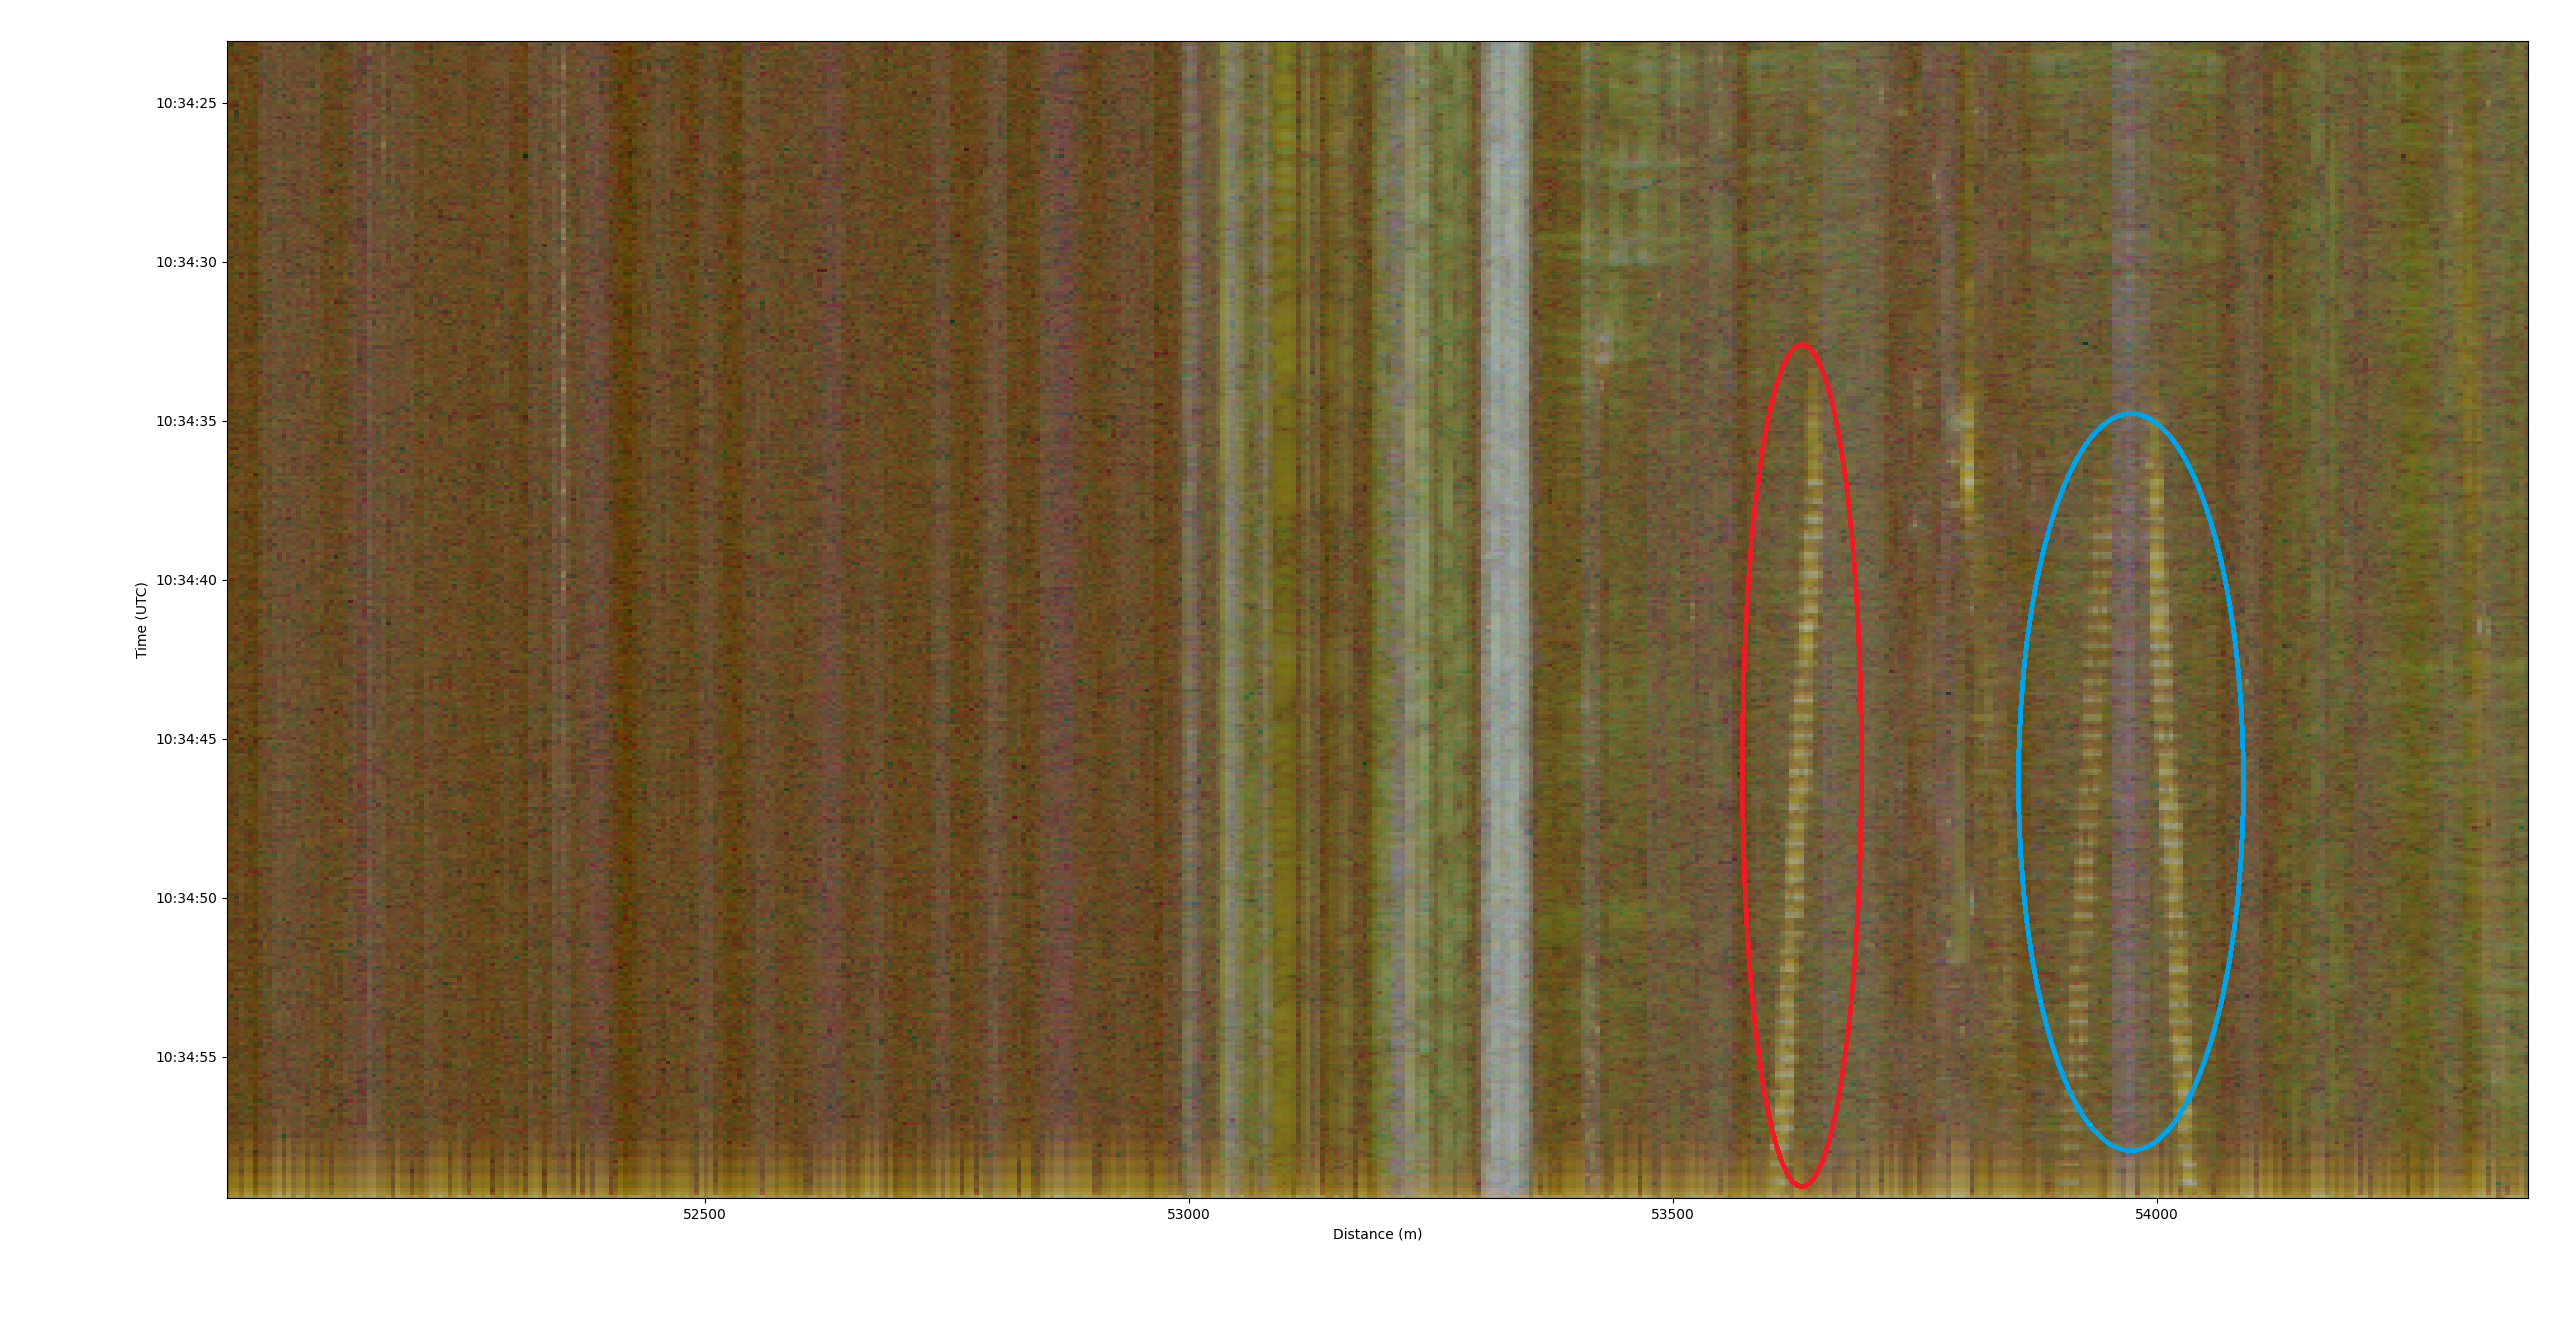
\includegraphics[width=\linewidth]{Bilder/jpg/plot_rgb.png}
    \caption{RGB plot for the phase data}
    \label{phase_plot}
\end{figure}

\subsection{Extraction}
\begin{figure}[ht]
  \centering
  \resizebox{\textwidth}{!}{%%
    \begin{tikzpicture}[
      node distance=1cm and 2cm,
      >=Stealth,
      subblock/.style={
        rectangle,
        draw,
        rounded corners,
        text centered,
        minimum width=2.5cm,
        minimum height=0.8cm,
        font=\scriptsize,
        fill=blue!10,
      },
      container/.style={
        rectangle,
        draw,
        thick,
        rounded corners,
        fill=gray!20,
      }
    ]
      % declare background layer
      \pgfdeclarelayer{background}
      \pgfsetlayers{background,main}

      % internal sub-blocks stacked
      \node[subblock] (hdf5) {HDF5 File};
      \node[subblock, below=of hdf5] (masks) {Region Masks};
      % output block
      \node[subblock, right=of masks] (steps) {Footstep and Background Files};

      % arrows from inputs to output
      \draw[->] (hdf5.east) -- ++(0.5,0) |- (steps.west);
      \draw[->] (masks.east) -- ++(0.5,0) -- (steps.west);

      % container in background
      \begin{pgfonlayer}{background}
        \node[container, fit=(hdf5) (masks) (steps), inner sep=10pt] (extract) {};
        \node[anchor=north west, font=\scriptsize] at (extract.north west) {Extraction};
      \end{pgfonlayer}
    \end{tikzpicture}%%
  }
  \caption{Extraction block: HDF5 file and Region masks are used to extract footstep and background data.}
  \label{fig:extraction_block}
\end{figure}

Figure~\ref{fig:extraction_block} shows the internal structure of extraction block which serves to isolate and package all footstep and background segments for downstream processing. It takes two simple inputs the raw phase data stored in the HDF5 file and the corresponding region masks and produces a set of cleaned, per event files. This abstract view hides the internal annotation details, focusing on the high-level data flow from stored measurements to ready to use footstep files.

\begin{figure}[ht]
  \centering
  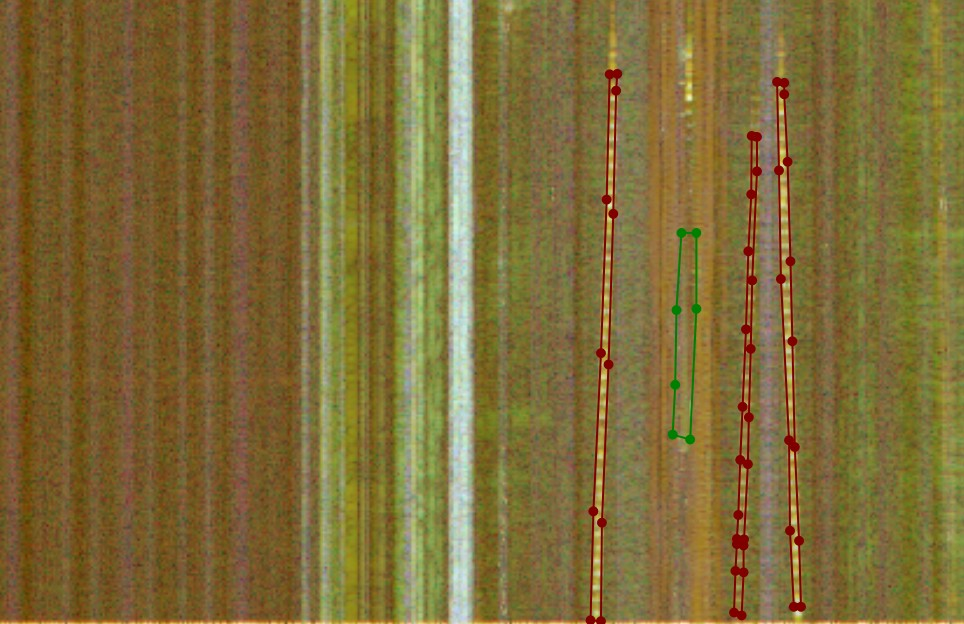
\includegraphics[width=\linewidth]{Bilder/jpg/labelme.jpg}
  \caption{Region annotation of background and footstep data}
  \label{labelme}
\end{figure}
 
Figure~\ref{labelme} shows the region masks for the annotation of the background and footstep data. The green annotation shows the background data and the red annotation shows the footsteps data. These annotations are used to store files in different folders such as background and walking. The annotation is done on the same HDF5 file shown in the Figure~\ref{phase_plot}.   

\subsection{Preprocessing}\label{sec:preprocessing}
The files generated from the extraction block need to be preprocessed in such a way that the footsteps are clearly visible. To help this cause, the preprocessing block converts the extracted files into spectrograms. The spectrograms are generated using the Short-Time Fourier Transform (STFT). Figure~\ref{fig:Preprocessing_block} shows the block diagram of the preprocessing block with all the operations done on the data files to get the spectrograms.

\begin{figure}[ht]
  \centering
  \resizebox{\textwidth}{!}{%%
    \begin{tikzpicture}[
      node distance=1cm,
      >=Stealth,
      subblock/.style={
        rectangle, draw, rounded corners, text centered,
        minimum width=2.5cm, minimum height=0.8cm,
        font=\scriptsize, fill=blue!10,
      },
      container/.style={
        rectangle, draw, thick, rounded corners, fill=gray!20,
      }
    ]
      % layers
      \pgfdeclarelayer{background}
      \pgfsetlayers{background,main}

      % sub-blocks inside
      \node[subblock] (acc) {Accumulator};
      \node[subblock, right=of acc] (stft) {STFT};
      \node[subblock, right=of stft] (spec) {Spectrogram};

        % Draw arrows
      \draw[->] (acc) -- (stft);
      \draw[->] (stft) -- (spec);

      % container background
      \begin{pgfonlayer}{background}
        \node[container, fit=(acc) (stft) (spec), inner sep=10pt] (prep) {};
        \node[anchor=north west, font=\scriptsize] at (prep.north west) {Preprocessing};
      \end{pgfonlayer}
    \end{tikzpicture}%%
  }
  \caption{Preprocessing block: Footstep/Background files are processed through an Accumulator and STFT to produce Spectrograms.}
  \label{fig:Preprocessing_block}
\end{figure}

Extracted data files from the extraction block are passed to the preprocessing block. Accumulator block takes the data files and integrates the phase-difference stream into a continuos phase signal and then the high-pass filters out slow drifts in such a way that only dynamic events like footsteps are visible. The STFT block takes this accumulated phase and converts it into a spectrogram. STFT is a mathematical technique that transforms the time-domain signal into the frequency domain, allowing for the analysis of the signal's frequency content over time. The output of the STFT is a spectrogram which is a visual representation of the signal's frequency content over time. Figure~\ref{walking_1d} shows such spectrogram which is generated from the footsteps data. The spikes seen in the spectrogram are the footsteps which are clearly visible. 

\begin{figure}[h]
  \centering
  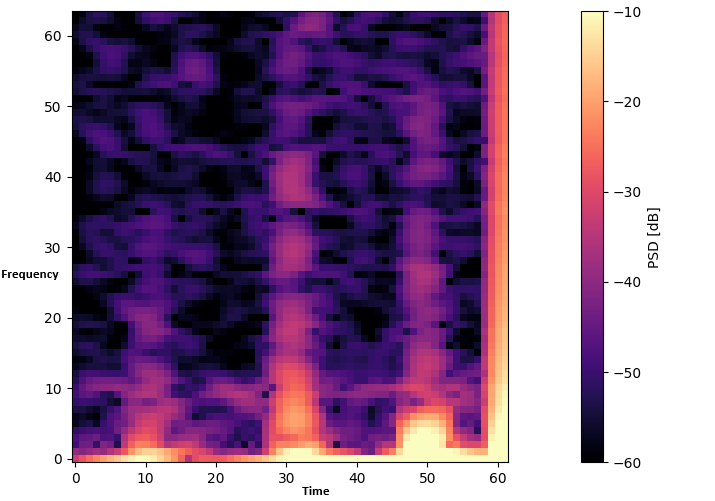
\includegraphics[width=0.7\linewidth]{Bilder/jpg/walking_1d.png}
  \caption{Spectrogram for walking data}
  \label{walking_1d}
\end{figure}

Background noise is also be visualized in the spectrograms in a similar manner. Figure~\ref{bg_1d} shows the spectrogram for background noise data. The spectrograms has no pattern of footsteps here. The pattern of footsteps has spikes but background noise will have a constant pattern which doesn't have distortions. The footsteps will have a significant spikes in the spectrograms unlike the background noise. This is a clear distinction between the footsteps and background noise spectrograms. 

\begin{figure}[h]
  \centering
  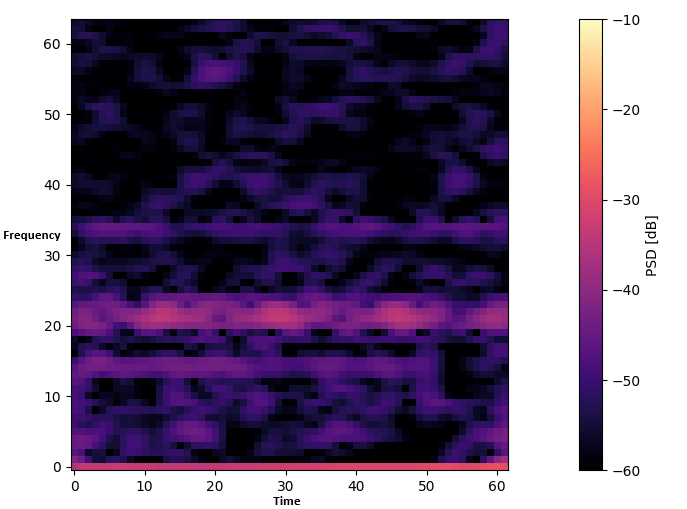
\includegraphics[width=0.7\linewidth]{Bilder/jpg/background_1d.png}
  \caption{Spectrogram for background noise data}
  \label{bg_1d}
\end{figure}

\subsection{Training the model}
Dataset created from the preprocessing block contains the footstep data and background data. Training block takes the dataset and trains the model using the ConvNext V2 and EfficientNet models. Figure~\ref{fig:training_block} shows the block diagram of the training pipeline.
\begin{figure}[ht]
  \centering
  \resizebox{\textwidth}{!}{%%
    \begin{tikzpicture}[
      node distance=1cm and 1.5cm,
      >=Stealth,
      subblock/.style={
        rectangle, draw, rounded corners, text centered,
        minimum width=3cm, minimum height=1cm,
        font=\scriptsize, fill=blue!10,
      },
      container/.style={
        rectangle, draw, thick, rounded corners, fill=gray!20,
      }
    ]
      % layers
      \pgfdeclarelayer{background}
      \pgfsetlayers{background,main}

      % Sub-blocks: first row
      \node[subblock] (dataset) {Dataset};
      \node[subblock, right=of dataset] (split) {Train/Val Split};
      \node[subblock, right=of split] (aug)   {Augmentation};
      % second row
      \node[subblock, below=of aug] (train) {Training};
      \node[subblock, left=of train] (val)   {Validation};
      \node[subblock, left=of val] (ckpt)   {Checkpoint};

      % Arrows
      \draw[->] (dataset) -- (split);
      \draw[->] (split) -- (aug);
      \draw[->] (aug.south) -- (train.north);
      \draw[->] (train) -- (val);
      \draw[->] (val) -- (ckpt);

      % Container background
      \begin{pgfonlayer}{background}
        \node[container, fit=(dataset) (split) (aug) (train) (val) (ckpt), inner sep=10pt] (trainC) {};
        \node[anchor=north west, font=\scriptsize] at (trainC.north west) {Training};
      \end{pgfonlayer}
    \end{tikzpicture}%%
  }
  \caption{Model training block: Footstep/Background dataset is split into training and validation sets, augmented, and then trained and validated.}
  \label{fig:training_block}
\end{figure}

The dataset consists of the spectrograms of footstep and background data. The dataset is split into training and validation sets in the ratio of 80:20. Training set is being applied augmentations to generalize the dataset so the model learns the features of the dataset and not memorize the dataset. The augmentations are explained in the section~\ref{sec:augmentation}. Training set is then passed to the model for training. Model is validated by just passing the validation set to the model. Model is trained and the checkpoint is saved. Checkpoint is the model weights which are saved after every epoch The model is then tested using the test set which is not used for training or validation. Test set is used to evaluate the performance of the model. Test set is passed to the model and the accuracy of the model is calculated using the checkpoint saved during the training. Testing follows the same process as validation, but done on the test set.  
